\chapter{数据预处理与数据增强}
数据是机器学习三要素之一,它决定了机器学习算法能达到的上限。对数据进行预处理与增强能有效提高模型性能,使用数据增强可扩充数据集防止过拟合。

入侵检测任务的目标是找到一种函数,该函数对于给定的序列$ \mathbf{X} = (\mathbf{x}_1, \mathbf{x}_2, \ldots, \mathbf{x}_n) $可以输出该序列每一个位置对应的类别$ \mathbf{Y} = (\mathbf{y}_1, \mathbf{y}_2, \ldots, \mathbf{y}_n) $。序列中的每一项代表一个数据包原始数据,每个数据包对应的信息是以二进制比特流形式呈现。由于二进制比特流不是定长的,且现在网络流量中大部分数据载荷都经过加密处理,如果直接分析加密的流量很难得到有效信息,且占较大存储空间。

因此部分数据集以统计特征形式给出而不是原始网络流。即采用统计学方法提取网络流量数据的统一特征,将变长的数据流转化为定长的统计特征向量。于是上文所说的给定序列中每一项$\mathbf{x}_i$就代表一个维度固定的向量。这些向量中既包含数值信息(如数据包的长度),也包含文本信息(如数据包的类型,TCP还是UDP)。包含文本信息的向量无法由机器学习模型直接处理,且一些数值分布范围广,给机器学习造成了困难。

本章提出的预处理方法,解决了上述问题。首先将数值替换文本,使该向量变成统一类型的向量,同时建立嵌入向量表,数值即为嵌入向量表中的索引。然后对原向量中的数值部分进行重新映射,将分布范围过大的数据项映射为分布范围较小的数据项,以便模型处理。

对网络流量进行时序建模时,还需要对流量数据进行切片。对切片后的数据进行数据增强,还需考虑维持原有数据分布及数据特点。
\section{入侵检测数据集}
研究中使用的数据集有两个,分别是KDDCUP-99和CIC-IDS2017\cite{Sharafaldin2018TowardGA},前者主要用于验证迁移学习性能,后者用于验证模型性能。
\subsection{KDDCUP-99数据集简介}

在入侵检测领域最基础的数据集是KDDCUP-99,这是一个竞赛数据集,该竞赛的任务是创建一个分类器以区分网络流量的好与坏。KDDCUP-99分为训练集与测试集,其中训练集包含七周的网络流量数据,有约500万条连接,测试集中包含两周的网络流量,大约包含200万条连接。每条连接指的是从tcp连接到释放连接的全部数据包序列。连接分为5个大类:
\begin{enumerate}
\item 正常流量:没有恶意的正常网络活动。
\item 拒绝服务(Denial-of-Service):发送大量无用信息,以耗尽服务器资源的网络活动。
\item 远程未授权访问(R2L):未经授权的用户通过远程访问获取资源,这种类型的网络流量通常用于窃取数据与破坏系统。
\item 本地未授权访问(U2R):攻击者试图在本地系统上获得超级用户的权限,一旦获取超级用户权限就可控制整个系统,并进一步进行攻击。
\item 探测(Probe):获取目标网络的当前状态,如开放端口以及正在运行的网络服务,识别可能存在漏洞,以方便进行下一步攻击。
\end{enumerate}

KDDCUP-99中的攻击类型分类情况如表\ref{table:kdd_attack_types}示,共7大类,15小类。标签数量如图\ref{fig:kdd99_category}示,可以看到拒绝服务流量最多,其次是正常流量,最少的是本地未授权访问。

\begin{table}[htb]
  \centering
  \caption{KDDCUP-99攻击类型总结}
  \begin{tabular}{p{0.15\linewidth}p{0.85\linewidth}}
    \toprule
    \textbf{攻击分类}& \textbf{具体类别}\\
    \midrule
    BENIGN & normal \\
    Denial-of-Service & back, neptune, smurf, teardrop, land, pod, apache2, mailbomb, processtable \\
    Probe & satan, portsweep, ipsweep, nmap, mscan, saint \\
    R2L & warezmaster, warezclient, ftp\_write, guess\_passwd, imap, multihop, phf, spy, sendmail, named, snmpgetattack, snmpguess, xlock, xsnoop, worm \\
    U2R & rootkit, buffer\_overflow, loadmodule, perl, httptunnel, ps, sqlattack, xterm \\
    \bottomrule
  \end{tabular}
  \label{table:kdd_attack_types}
\end{table}

\begin{figure}[htb]
\centering % 居中对齐子图
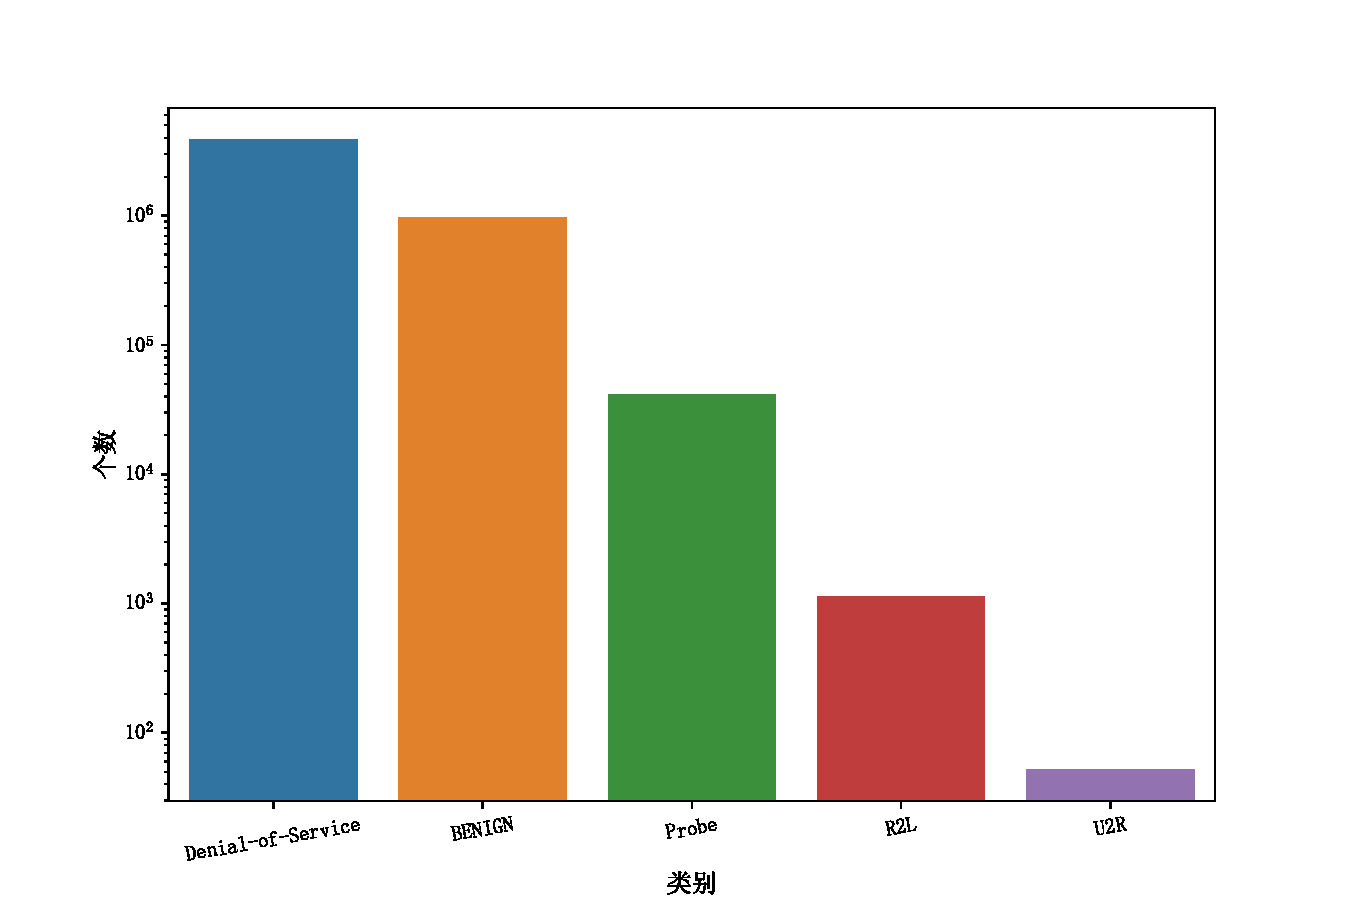
\includegraphics[width=.95\linewidth]{img/preprocessing/kdd99_category.pdf} % 插入SVG图片
\caption{KDDCUP-99类别分布}
\label{fig:kdd99_category} % 子图的标签,用于交叉引用
\end{figure}%

\subsection{CIC-IDS2017数据集简介}
CIC-IDS2017是另一个网络入侵检测领域常用的数据集,该数据集采集自5天的网络流量,既包含原始数据,也包含使用CICFlowMeter分析后的结果。数据集没有划分训练集与测试集,共3119345条数据。数据分为7个大类:
\begin{enumerate}
\item 正常流量:没有恶意的正常网络活动。
\item 暴力攻击:攻击者尝试用户名以及密码,通过认证从而获取权限。
\item 机器人网络:攻击者通过控制大量机器组成攻击平台,可对攻击目标产生巨大的攻击流量。
\item 端口扫描:识别当前网络开放的端口,确定服务器上正在运行的服务与应用。
\item 拒绝服务:攻击者建立大量半开连接从而消耗服务器资源,阻碍服务器对正常请求的响应。
\item 网络应用程序攻击:此类攻击主要指因程序设计不合理,导致服务器无法区分命令与数据的攻击类型,如各种注入攻击。
\item 未知类型:主要指难以确定的小样本攻击类型。
\end{enumerate}

CIC-IDS2017攻击类型分类情况如表\ref{table:cic2017_attack_types}示,共7大类,24小类。标签数量如图\ref{fig:cic2017_category}示,可以看到正常流量最多;其次是拒绝服务、端口扫描和暴力攻击,这些攻击类型本身就需要大量的攻击流量,然后是网络应用攻击和机器人网络,最少的是未知类型攻击,在对数坐标系下也显著少于其他类型。

\begin{table}[htb]
  \centering
  \caption{KDDCUP-99攻击类型总结}
  \begin{tabular}{p{0.2\linewidth}p{0.8\linewidth}}
    \toprule
    \textbf{攻击类型(大类)} & \textbf{攻击类型(小类)} \\
    \midrule
    BENIGN & BENIGN \\
    Brute-force-attack & FTP-Patator, SSH-Patator \\
    Botnet & Bot \\
    Denial-of-Service & DoS GoldenEye, DoS Hulk, DoS Slowhttptest, DoS slowloris, DDoS \\
    Web-Attacks & Web Attack – Brute Force, Web Attack – Sql Injection, Web Attack – XSS \\
    PortScan & PortScan \\
    Unknown & Infiltration, Heartbleed \\
    \bottomrule
  \end{tabular}
  \label{table:cic2017_attack_types}
\end{table}
\begin{figure}[htb]
\centering % 居中对齐子图
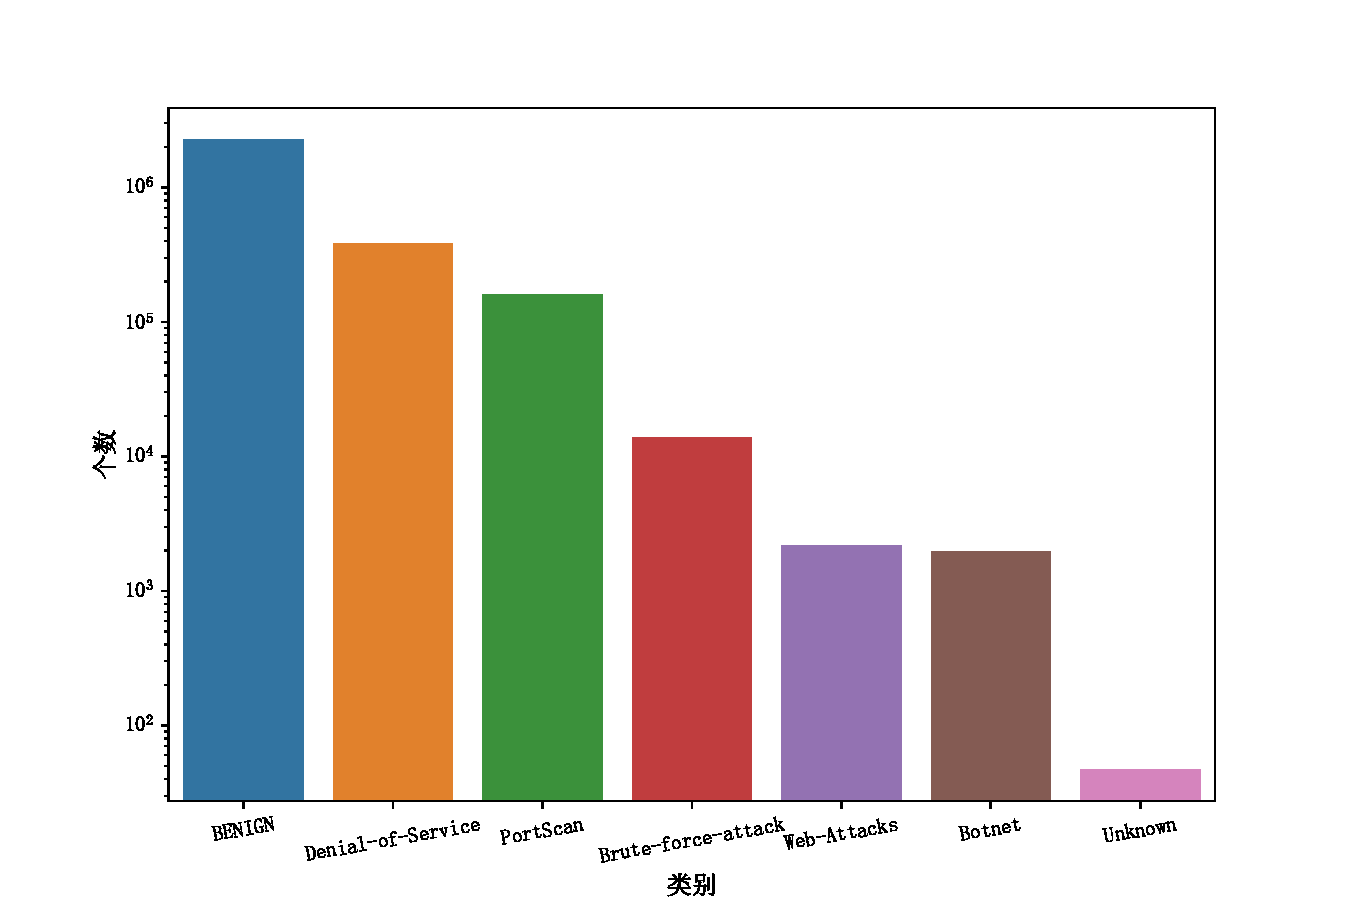
\includegraphics[width=.95\linewidth]{img/preprocessing/cic2017_category.pdf} % 插入SVG图片
\caption{CIC-IDS2017类别分布}
\label{fig:cic2017_category} % 子图的标签,用于交叉引用
\end{figure}%

\section{数据集格式}
网络入侵检测数据通常有两种格式,分别是原始捕获的二进制比特流以及通过如CICFlowMeter等网络流量分析工具初步分析后得到的统计特征,KDDCUP-99数据集只给出了统计特征,CIC-IDS2017数据集给出了这两者,为了形式统一,本研究仅使用流量分析工具得到的统计特征。
\subsection{KDDCUP-99数据集格式}
KDDCUP-99数据集是以逗号分隔符形式给出的,可以看作是一张表格,总共42列,前41列是连接的特征,最后一列是连接的类别,数据集共4898431行。第1行数据如下:
\begin{itemize}
\item \seqsplit{0,tcp,http,SF,215,45076,0,0,0,0,0,1,0,0,0,0,0,0,0,0,0,0,1,1,0.00,0.00,0.00,0.00,1.00,0.00,0.00,0,0,0.00,0.00,0.00,0.00,0.00,0.00,0.00,0.00,normal.}
\end{itemize}
这41列特征按数值类型可分为四类,分别是:表示是与否的二值类型、表示百分比的浮点类型、表示文本的字符串、表示个数的整数值,其中二值类型可看作特殊的百分比,41维特征划分如表\ref{table:kdd_feature_types}示。

\begin{table}[htbp]
\centering
\caption{数据类型分类}
\begin{tabular}{p{0.15\linewidth}p{0.7\linewidth}}
\toprule
\textbf{类型} & \textbf{名称} \\
\midrule
整数 & duration, src\_bytes, dst\_bytes, land, wrong\_fragment, urgent, hot, num\_failed\_logins, lnum\_compromised, lnum\_root, lnum\_file\_creations, lnum\_shells, lnum\_access\_files, lnum\_outbound\_cmds, count, srv\_count, dst\_host\_count, dst\_host\_srv\_count \\
\addlinespace
浮点或二值 & logged\_in, lroot\_shell, lsu\_attempted, is\_host\_login, is\_guest\_login, serror\_rate, srv\_serror\_rate, rerror\_rate, srv\_rerror\_rate, same\_srv\_rate, diff\_srv\_rate, srv\_diff\_host\_rate, dst\_host\_same\_srv\_rate, dst\_host\_diff\_srv\_rate, dst\_host\_same\_src\_port\_rate, dst\_host\_srv\_diff\_host\_rate, dst\_host\_serror\_rate, dst\_host\_srv\_serror\_rate, dst\_host\_rerror\_rate, dst\_host\_srv\_rerror\_rate \\
\addlinespace
文本 & protocol\_type, service, flag \\
\bottomrule
\end{tabular}
\label{table:kdd_feature_types}
\end{table}

整数类型含义指某种操作的次数包的个数长度等,将这类数值进行可视化如图\ref{fig:kdd99_bighist}示,可见其分布不均,大部分数值较小。

百分比类型含义指连接中某类连接占总连接的百分比或者某种操作是否成功,分别对二者类型百分比类型以及两者合并后的数值进行可视化分析,如图示\ref{fig:kdd99_samllhist},等于0与等于1的值最多。

文本类型包括协议类型,网络服务类型以及连接的状态。

\begin{figure}[htbp] % 创建一个新的figure环境
\centering % 居中对齐所有的子图

\subfloat[分布范围小的属性分布情况]{ % 插入第一个子图及其标题
\begin{minipage}{.5\textwidth}
\centering % 居中对齐子图
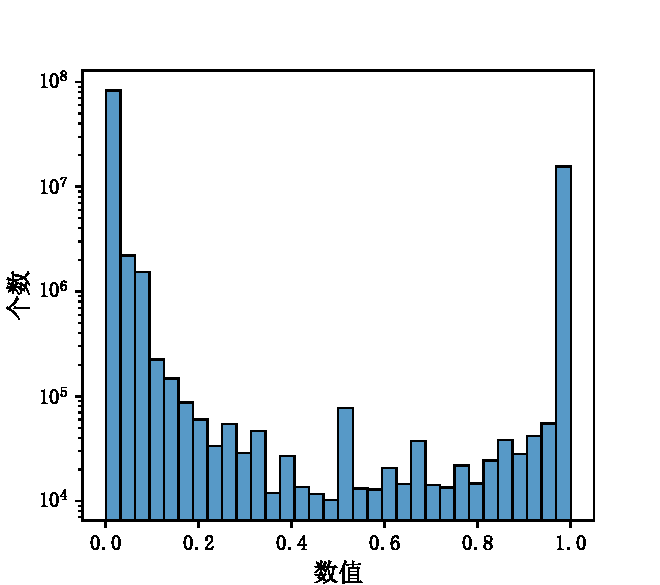
\includegraphics[width=1\linewidth]{img/preprocessing/kdd99_smalldata.pdf} % 插入SVG图片
\label{fig:kdd99_samllhist} % 子图的标签,用于交叉引用
\end{minipage}%
}
\subfloat[分布范围大的属性分布情况]{ % 插入第二个子图及其标题
\begin{minipage}{.5\textwidth}
\centering
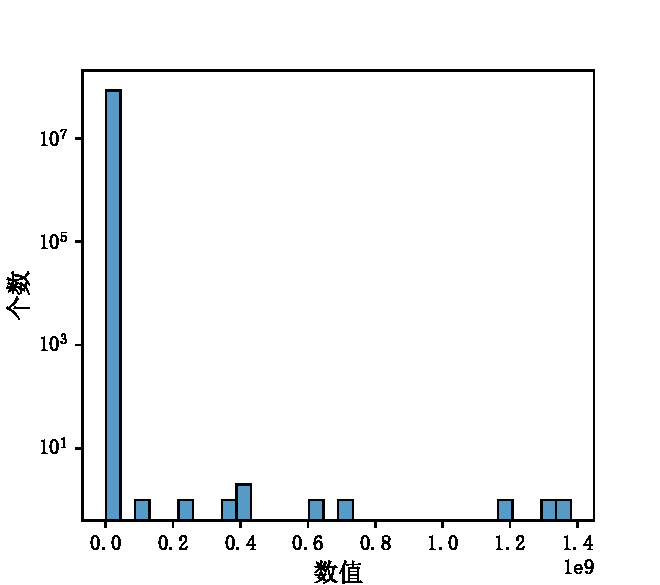
\includegraphics[width=1\linewidth]{img/preprocessing/kdd99_bigdata.pdf} % 插入SVG图片
\label{fig:kdd99_bighist}
\end{minipage}
}

\caption{kdd99数据(正数部分)分布直方图} % 四张图片作为整体的标题
\label{fig:kdd99_hist}
\end{figure}


\subsection{CIC-IDS2017数据集格式}

该数据集以逗号分隔符形式给出,有多个文件,总共85列,第1列是连接的特征码由连接双方的IP地址端口以及协议类型组成,有两列列名为“Fwd Header Length”重复的列,最后一列是连接的类别,其他的82列为连接特征。第1行数据如下:
\begin{itemize}
\item \seqsplit{192.168.10.5-8.254.250.126-49188-80-6,8.254.250.126,80,192.168.10.5,49188,6,03/07/2017 08:55:58,4,2,0,12.0,0.0,6.0,6.0,6.0,0.0,0,0,0,0,3000000.0,500000.0,4.0,0.0,4.0,4.0,4.0,4.0,0.0,4.0,4.0,0,0,0,0,0,0,0,0,0,40,0,500000.0,0.0,6.0,6.0,6.0,0.0,0.0,0,0,0,0,1,1,0,0,0.0,9.0,6.0,0.0,40,0,0,0,0,0,0,2,12,0,0,329,-1,1,20,0,0,0,0,0,0,0,0,BENIGN}
\end{itemize}
连接特征中的双方IP地址、时间戳无法用于分类。故可用于分类的特征有79列,按数值范围和类型可分为三类,分别是:表示索引的数值,最大值小于等于1的数值,最大值大于1的数值,79维特征划分如表\ref{table:cic2017_feature_types}示。

\begin{table}[htb]
\centering
\caption{数据类型分类}
\begin{tabular}{p{0.15\linewidth}p{0.57\linewidth}}
\toprule
\textbf{类型} & \textbf{名称} \\
\midrule
最大值大于1 & Flow Duration, Total Fwd Packets, Total Backward Packets, Total Length of Fwd Packets, Total Length of Bwd Packets, Fwd Packet Length Max, Fwd Packet Length Min, Fwd Packet Length Mean, Fwd Packet Length Std, Bwd Packet Length Max, Bwd Packet Length Min, Bwd Packet Length Mean, Bwd Packet Length Std, Flow Bytes/s, Flow Packets/s, Flow IAT Mean, Flow IAT Std, Flow IAT Max, Flow IAT Min, Fwd IAT Total, Fwd IAT Mean, Fwd IAT Std, Fwd IAT Max, Fwd IAT Min, Bwd IAT Total, Bwd IAT Mean, Bwd IAT Std, Bwd IAT Max, Bwd IAT Min, Fwd Header Length, Bwd Header Length, Fwd Packets/s, Bwd Packets/s, Min Packet Length, Max Packet Length, Packet Length Mean, Packet Length Std, Packet Length Variance, Down/Up Ratio, Average Packet Size, Avg Fwd Segment Size, Avg Bwd Segment Size, Subflow Fwd Packets, Subflow Fwd Bytes, Subflow Bwd Packets, Subflow Bwd Bytes, Init\_Win\_bytes\_forward, Init\_Win\_bytes\_backward, act\_data\_pkt\_fwd, min\_seg\_size\_forward, Active Mean, Active Std, Active Max, Active Min, Idle Mean, Idle Std, Idle Max, Idle Min\\
\addlinespace
最大值小于1 & Fwd PSH Flags, Bwd PSH Flags, Fwd URG Flags, Bwd URG Flags, FIN Flag Count, SYN Flag Count, RST Flag Count, PSH Flag Count, ACK Flag Count, URG Flag Count, CWE Flag Count, ECE Flag Count, Fwd Avg Bytes/Bulk, Fwd Avg Packets/Bulk, Fwd Avg Bulk Rate, Bwd Avg Bytes/Bulk, Bwd Avg Packets/Bulk, Bwd Avg Bulk Rate \\
\addlinespace
索引值 & Source Port, Destination Port, Protocol \\
\bottomrule
\end{tabular}
\label{table:cic2017_feature_types}
\end{table}

分布范围小于等于1的数值指连接中是否存在FIN、SYN、ACK等标识或者是表示某种占比,如图\ref{fig:cic2017_samllhist}示,可见其分布范围集中于0附近与1附近,实际上尽管某些属性表示占比,但这些属性只有0和1两个值,且0的个数远大于1的个数。

分布范围大的数值含义指某种操作的次数、包的个数、包的长度等,将这类数值进行可视化如图\ref{fig:cic2017_bighist}示,可以看出其分布不均,绝大多数数值较小,数据分布范围广。

索引的数值表示端口号或协议号。

\begin{figure}[htbp] % 创建一个新的figure环境
\centering % 居中对齐所有的子图

\subfloat[分布范围小的属性分布情况]{ % 插入第一个子图及其标题
\begin{minipage}{.5\textwidth}
\centering % 居中对齐子图
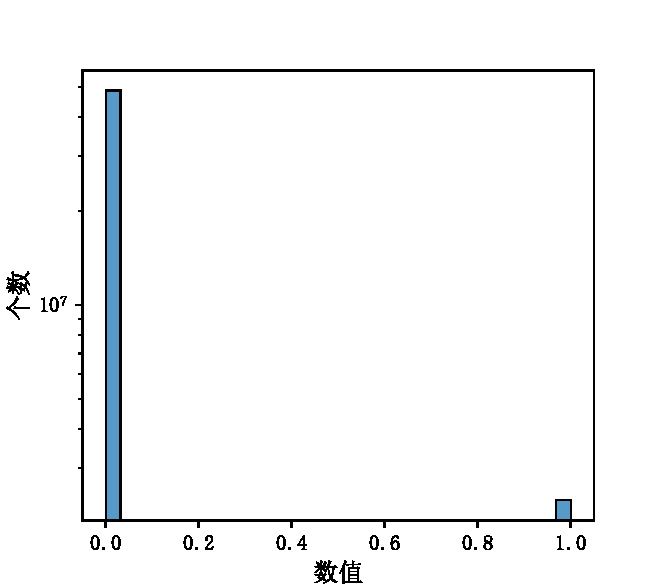
\includegraphics[width=1\linewidth]{img/preprocessing/cic2017_smalldata.pdf} % 插入SVG图片
\label{fig:cic2017_samllhist} % 子图的标签,用于交叉引用
\end{minipage}%
}
\subfloat[分布范围大的属性分布情况]{ % 插入第二个子图及其标题
\begin{minipage}{.5\textwidth}
\centering
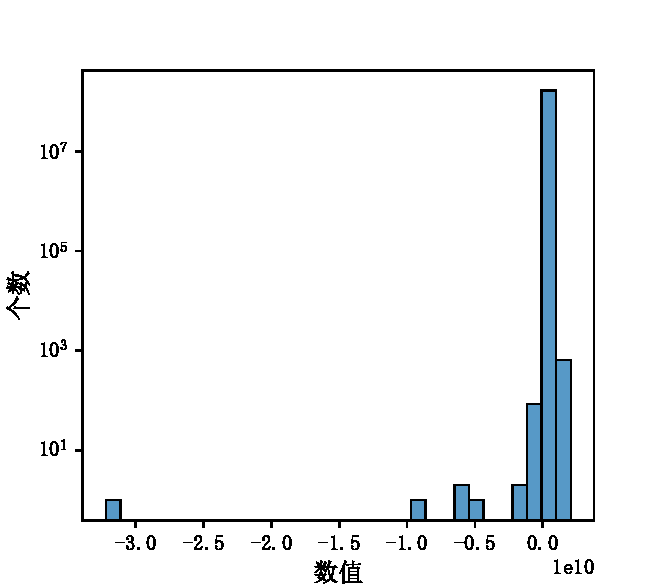
\includegraphics[width=1\linewidth]{img/preprocessing/cic2017_bigdata.pdf} % 插入SVG图片
\label{fig:cic2017_bighist}
\end{minipage}
}

\caption{CIC-IDS2017数据(正数部分)分布直方图} % 四张图片作为整体的标题
\label{fig:cic2017_hist}
\end{figure}

\section{数据预处理}
\subsection{数据清洗}
常见的数据集并不是规范的。

第一步是规范化整体数据,首先移除重复的列,然后查找数据中存在缺失数据的行,将这些行移除。

第二步是规范化数值类型,考虑到数据集中数值类型分布范围广,本章通过提出新的标准化算法,缩小数据分布范围,方便模型学习。

第三步是规范化非数值类型,对于非数值属性如协议类型,在不同数据集上可能是文本形式,也可能是协议代号形式,同一意义的不同格式数据会给模型学习带来困难,因此需要将其转为统一格式。


\subsection{数据转换}
\subsubsection{数值转换}

数据集中提供的数据包括均值、方差、包长度、字节数等。其中,一些数据,例如src\_bytes(从源主机到目标主机的数据字节数),其分布范围过大,不利于后续神经网络的处理。因此采用了以下算法\ref{alg:map_gt1},对分布范围大于1的属性值进行重新映射,以缩小分布范围。

映射前后数值分布情况如图\ref{fig:transf_hist}示。映射前分布不均,大部分数值分布在0附近,少部分数值较大,存在极少数负值,且负值分布极为稀疏。

映射后分布明显均匀,负数部分分布稀疏形况得到改善,正数部分分布更均匀,整体分布范围显著缩小,从十亿级别的分布变为-30至25之间,利于模型区分其中较小的数值差异。

\begin{figure}[htbp] % 创建一个新的figure环境
\centering % 居中对齐所有的子图

\subfloat[数据转换前分布情况]{ % 插入第一个子图及其标题
\begin{minipage}{.5\textwidth}
\centering % 居中对齐子图
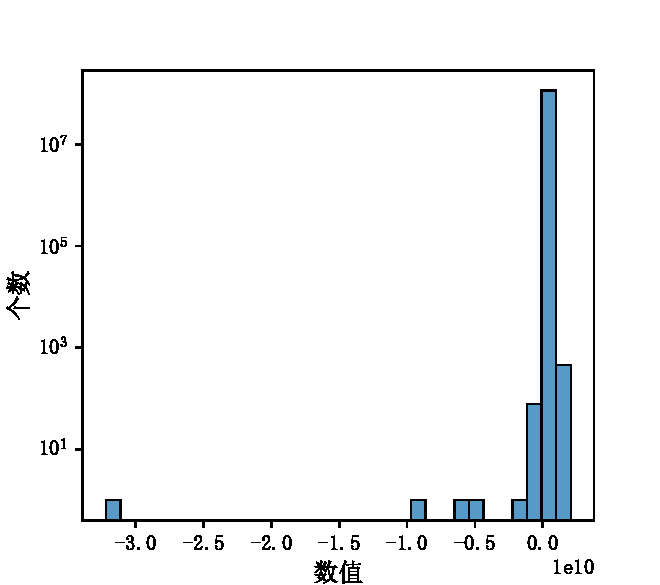
\includegraphics[width=1\linewidth]{img/preprocessing/logtransf_before.pdf} % 插入SVG图片
\label{fig:logtransf_before} % 子图的标签,用于交叉引用
\end{minipage}%
}
\subfloat[数据转换后分布情况]{ % 插入第二个子图及其标题
\begin{minipage}{.5\textwidth}
\centering
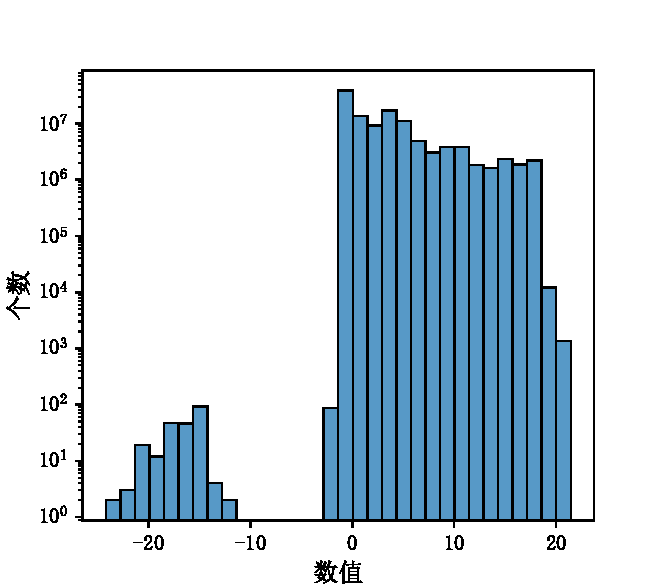
\includegraphics[width=1\linewidth]{img/preprocessing/logtransf_after.pdf} % 插入SVG图片
\label{fig:logtransf_after}
\end{minipage}
}

\caption{数值转换前后分布直方图} % 四张图片作为整体的标题
\label{fig:transf_hist}
\end{figure}

\begin{algorithm}[htbp]
\caption{数据预处理算法}
\begin{algorithmic}
\REQUIRE 矩阵 $A$
\ENSURE 处理后的矩阵 $B$
\STATE \textbf{步骤 1:} 对矩阵 $A$ 的每一列求绝对值的最大值
\FOR{每一列 $j$}
    \STATE $maxValue \gets 0$
    \FOR{每一行 $i$}
        \STATE $maxValue \gets \max(maxValue, |A_{i,j}|)$
    \ENDFOR
    \STATE $B_{*,j} \gets maxValue$
\ENDFOR
\STATE \textbf{步骤 2:} 筛选出最大值大于 1 的列
\STATE $selectedColumns \gets \emptyset$
\FOR{每一列 $j$}
    \IF{$B_{*,j} > 1$}
        \STATE $selectedColumns \gets selectedColumns \cup \{j\}$
    \ENDIF
\ENDFOR
\STATE \textbf{步骤 3:} 对筛选出的列,保留原符号,对其绝对值取对数
\FOR{每一列 $j \in selectedColumns$}
    \FOR{每一行 $i$}
        \STATE $B_{i,j} \gets \mathrm{sign}(A_{i,j}) \cdot \log(|A_{i,j}|)$
    \ENDFOR
\ENDFOR
\end{algorithmic}
\label{alg:map_gt1}
\end{algorithm}



\subsubsection{非数值转换}
本节定义的统一格式是文本形式。对于网络协议,会构建一个协议号至描述的映射表,从而将协议代号后转化为其对应的描述,过程如图\ref{fig:convert_ipport}示。

端口号的映射则较为复杂,一些网络服务有固定的端口号,但同一端口不同协议如TCP或UDP其对应的意义并不相同。因此需要构建二元组(端口号,协议)至描述的映射表,该映射表可准确地将端口号转化为其对应的描述,过程如图\ref{fig:convert_ipport}示。一般而言,服务器端的端口号是固定的,而客户端的端口号则不是固定的,因此需要将未进行映射的端口号描述置为“no available”,代表临时端口号。

\begin{figure}[htbp]
\centering % 居中对齐子图
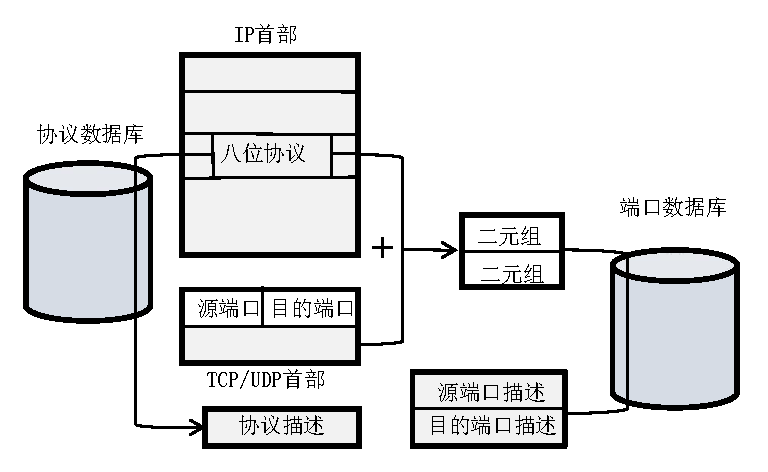
\includegraphics[width=1\linewidth]{img/preprocessing/convert_ipport.pdf} % 插入SVG图片
\caption{协议号与端口号转换过程}
\label{fig:convert_ipport} % 子图的标签,用于交叉引用
\end{figure}%

\subsection{数据切片与划分}
网络入侵检测数据集提供了连续的流量数据特征,模型无法处理过长的特征,因此需要将其进行切片。切片后需要对片段进行打乱,避免模型记忆序列本身而不是特征,同时还使不同类型的片段均匀分布。最后按比例将乱序片段划分为训练集与测试集,过程如图\ref{fig:divide_slice}示。

\begin{figure}[htbp]
\centering % 居中对齐子图
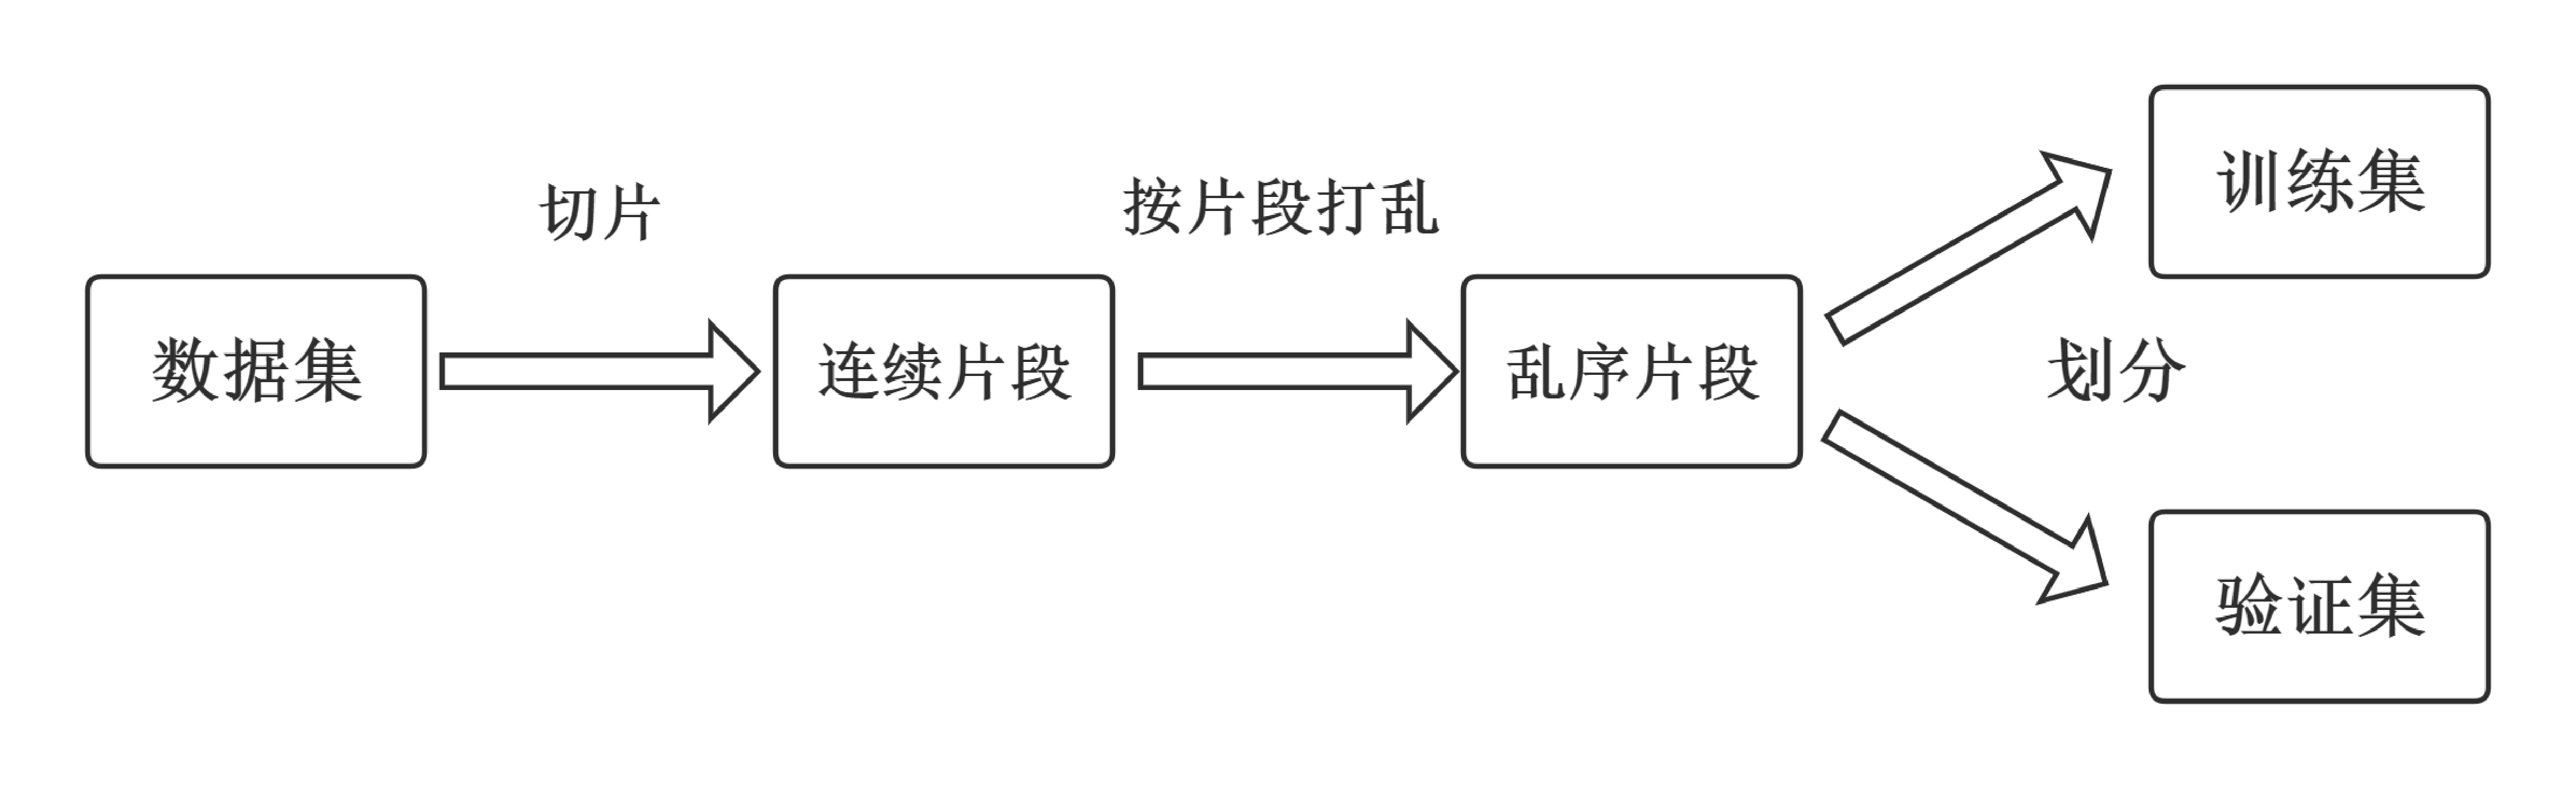
\includegraphics[width=1\linewidth]{img/preprocessing/divide_slice.pdf} % 插入SVG图片
\caption{数据集切片与划分过程}
\label{fig:divide_slice} % 子图的标签,用于交叉引用
\end{figure}%

\section{数据增强}
数据增强是机器学习中的常用技术,它通过数据集中已有样本合成新样本且新样本符合数据集中的数据分布。通过数据增强,扩充数据集大小,可以提高模型的泛化能力。若进行类别加权的数据增强,还可增加稀有样本出现频率以平衡数据集。

在上述处理过程中,为了实现时序建模,对数据集中连续的网络流量加窗,分割为长度相等的连接序列,该序列表示一段时间内网络连接情况。网络入侵检测中常见的数据增强方式是使用样本及其邻近样本重新合成新的数据,考虑到不同连接之间可能存在时间依赖关系,上述合成方式可能会破坏时间依赖关系,本章提出一种保持内部有序关系的序列数据增强算法\ref{algorithm:shuffle_data}。

\begin{algorithm}[htbp]
\caption{数据与固定标签的混洗算法}
\begin{algorithmic}
\REQUIRE 标签数组 $labels$
\ENSURE 根据标签混洗后的索引数组 $ans$,表示混洗后数组的新位置
\STATE \textbf{步骤 1:} 确定每个标签的索引位置
\STATE $unique\_labels, label\_positions \gets \mathrm{np.unique}(labels, \mathrm{return\_inverse=True})$
\STATE \textbf{步骤 2:} 为每个标签生成一个随机序列
\STATE $random\_label \gets \mathrm{np.random.permutation}(labels)$
\STATE \textbf{步骤 3:} 初始化一个与标签数组大小相同的索引数组
\STATE $shuffled\_indices \gets \mathrm{np.arange}(labels.size)$
\STATE $ans \gets shuffled\_indices.copy()$
\STATE \textbf{步骤 4:} 对于每个唯一标签,找到相应的数据索引并进行混洗
\FOR{每个标签 $label$ 在 $unique\_labels$ 中}
    \STATE $new\_mask \gets random\_label == label$
    \STATE $old\_mask \gets labels == label$
    \STATE $ans[new\_mask] \gets shuffled\_indices[old\_mask]$
\ENDFOR
\end{algorithmic}
\label{algorithm:shuffle_data}
\end{algorithm}


该算法的核心前提是不同类别之间的数据没有时间依赖。上述算法的核心在步骤四,普通混洗算法生成新元素的下标,本章提出的混洗算法则生成每个位置对应的类别。这一过程保证同一类别的数据虽然被映射到新位置,但其内部顺序仍然得以保持,从而维护了原数据中的时间依赖关系。

上述算法并没有直接生成新数据,而是生成增强后每个数据包的新位置。在保持时间依赖关系的情况下,增加数据多样性有助于提升模型的时序建模能力。


\section{本章小结}
本章主要介绍了所用的两种数据集,对每种数据集的特征进行分析。根据数据及特点进行了数据清洗、数值转换、数据切片过程,实现了数据的缩放,对网络流量中的非数值特征部分提出了一种新的转换方式,将先验知识(文本描述)引入其中,同时实现了不同数据集之间描述的统一化。提出了一种新的数据增强方法,利用标签,不改变数据分布的情况下,获得多样性的数据。
